\documentclass[12pt]{article}
\begin{document}
\usepackage{mhchem}
\usepackage{graphicx}
\begin{itemize}
\item 
Swartz reaction is not a special case of Finkelstein reaction! One uses metallic flourides and the other uses just plain substitution{is also a equilibrium reaction}.

\item 
Route to convert iodide to chloride.
\[
\ce{RI ->[Strong base] ROH ->[NaI + Acetone] RI}
\]

\item
HBr shows markonikov addition without peroxides and shows anti-markonikov addition with peroxides

\item
N-Bromosuccinamide reaction is called Wohl–Ziegler reaction. It adds one bromine atom to a sp3 carbon atom just next to a sp2 carbon atom. 

\item
Molecules with greater molecular mass have stronger vander walls forces.

\item
Boiling point increases with increase in branching for isomeric alkanes

\item 
Boiling point is about intermolecular forces more while Melting point is about solid state packing and symmetry more

\item
There is possibility of backside attack in cyclohexyl compounds.

\item
	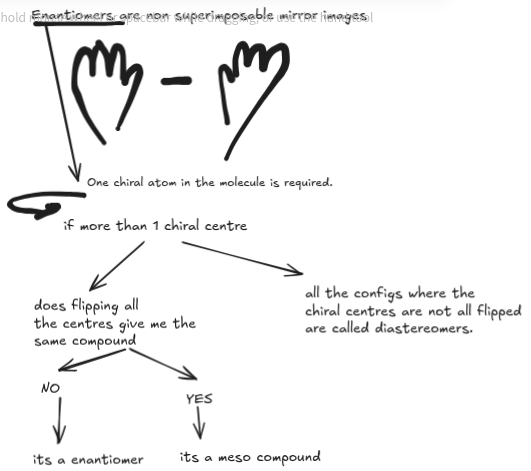
\includegraphics{Fig1.png}

\item
Nitrate salts are completely dissociable like strong electrolyte.

\item

